\documentclass[tikz=true, border=12pt]{standalone}
\begin{document}


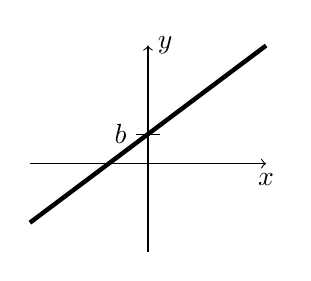
\begin{tikzpicture}[scale=0.75]
    \draw[white,fill=white] (-2,-1.5) rectangle (2.2,2.2);
          \draw[->] (-2,0) -- (2,0) node[below] {$x$};
          \draw[->] (0,-1.5) -- (0,2) node[right] {$y$};
          \draw[domain=-2:2,smooth,variable=\x,black,ultra thick] plot ({\x},{0.75*\x+0.5});
          \draw (0.2,0.5) -- (-0.2,0.5) node[left] {$b$};
          %\node at (4.5, 9.5){$y = 3x+4$};
          %\node at (3.5, 6.5){Slope = 3};
          %\node[right]at (0, 4){$4$};
          %\node[below] at (-1.33, 0) {$-\frac{4}{3}$};
        \end{tikzpicture}


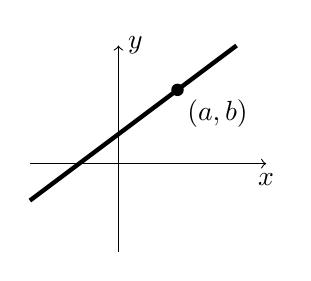
\begin{tikzpicture}[scale=0.75]
    \draw[white,fill=white] (-1.5,-1.5) rectangle (2.7,2.2);
            \draw[->] (-1.5,0) -- (2.5,0) node[below] {$x$};
            \draw[->] (0,-1.5) -- (0,2) node[right] {$y$};
            \draw[domain=-1.5:2,smooth,variable=\x,black,ultra thick] plot ({\x},{0.75*\x+0.5});
            %\draw (0.2,0.5) -- (-0.2,0.5) node[left] {$b$};
            \fill (1,1.25) circle [radius = 3pt] node[below right] {$(a,b)$};
            %\node at (4.5, 9.5){$y = 3x+4$};
            %\node at (3.5, 6.5){Slope = 3};
            %\node[right]at (0, 4){$4$};
            %\node[below] at (-1.33, 0) {$-\frac{4}{3}$};
        \end{tikzpicture}
            

\end{document}